\section{Introduction}
The Goertzel algorithm is a digital signal processing algorithm and an efficient convolutional variant of the discrete Fourier transform used for efficient detection of specific frequencies in a signal. The algorithm provides an efficient alternative to the fast Fourier transform (FFT) for applications that require only a few frequency components and it is mostly employed in DTMF systems (dual tone multi-frequency systems) as a tone detector.\\
The purpose of this report is to describe not only our implementation  of the Goertzel algorithm, but to also give an overview of the development process behind such implementation. In order to achieve this, this report will be structured in a way that reflects our process. Section n.\ref{sec:theory} describes the general theory of the filter, as it was essential for us to first gain an understanding of the characteristics of the algorithm. In Section n.\ref{sec:lit_ref} an overview of the state of the art will be given, where applications and different implementations of the algorithm will be discussed. The description of the implemented algorithm will be provided in Section n. \ref{sec:implementation}. The main goal was to provide a Goertzel algorithm implementation that is effective, optimized, and satisfies the required specifications. Furthermore, the implementation has to be done in such a way that it could be synthetized in an FPGA/ASIC platform. To confirm the behavioural correctness and accuracy of the Goertzel Filter implementation, a VHDL test bench will be created, and a MATLAB simulation will be used to generate the input stimulus data and expected outputs, which will be described in Section n. \ref{sec:simulation}. This simulation was used for various purposes, but mainly to refine the understanding of the algorithm, making design choices and to verify the accuracy of such design.
%\section{Project Scope}
%The Goertzel Filter design and implementation on an FPGA platform for frequency detection are included in the project's scope. The goal is to provide a Goertzel algorithm implementation that is effective, optimized, and satisfies the required specifications. The project's primary components will comprise the following: 
%\begin{itemize}
 %   \item Explore the Goertzel Filter: The Goertzel filter principle, a digital signal processing technique employed for identifying specific frequencies in a signal, will be comprehended as part of the project's objective. Moreover,the state-of-the-art applications of the Goertzel filter will be investigated. %, encompassing domains like speech recognition, telecommunications, and audio processing.
%\end{itemize}
%\begin{itemize}
 %   \item Design of a Goertzel filter: A Goertzel filter will be created using the requirements provided. The Goertzel algorithm for frequency detection will be implemented in the filter, which will be synthesizable and created to run on an FPGA / VLSI platform.
%\end{itemize}
%\begin{itemize}
 %   \item Goertzel Filter VHDL Implementation: VHDL will be used to implement the Goertzel Filter design. The Goertzel algorithm computations will be precisely carried out by the VHDL code, which will also interface with the required peripherals.
%\end{itemize}
%\begin{itemize}
 %   \item Development of a Test Bench: To confirm the behavioural correctness and accuracy of the Goertzel Filter implementation, a VHDL test bench will be created. MATLAB will be used to generate the input stimulus data and expected outputs. To verify the accuracy of the design, the Goertzel Filter's output results will be compared to those that were anticipated.
%\end{itemize}

%\begin{itemize}
    %\item Test Cases: A number of test cases will be developed to verify the functional correctness of the Goertzel Filter.
%\end{itemize}
\begin{figure}
    \centering
    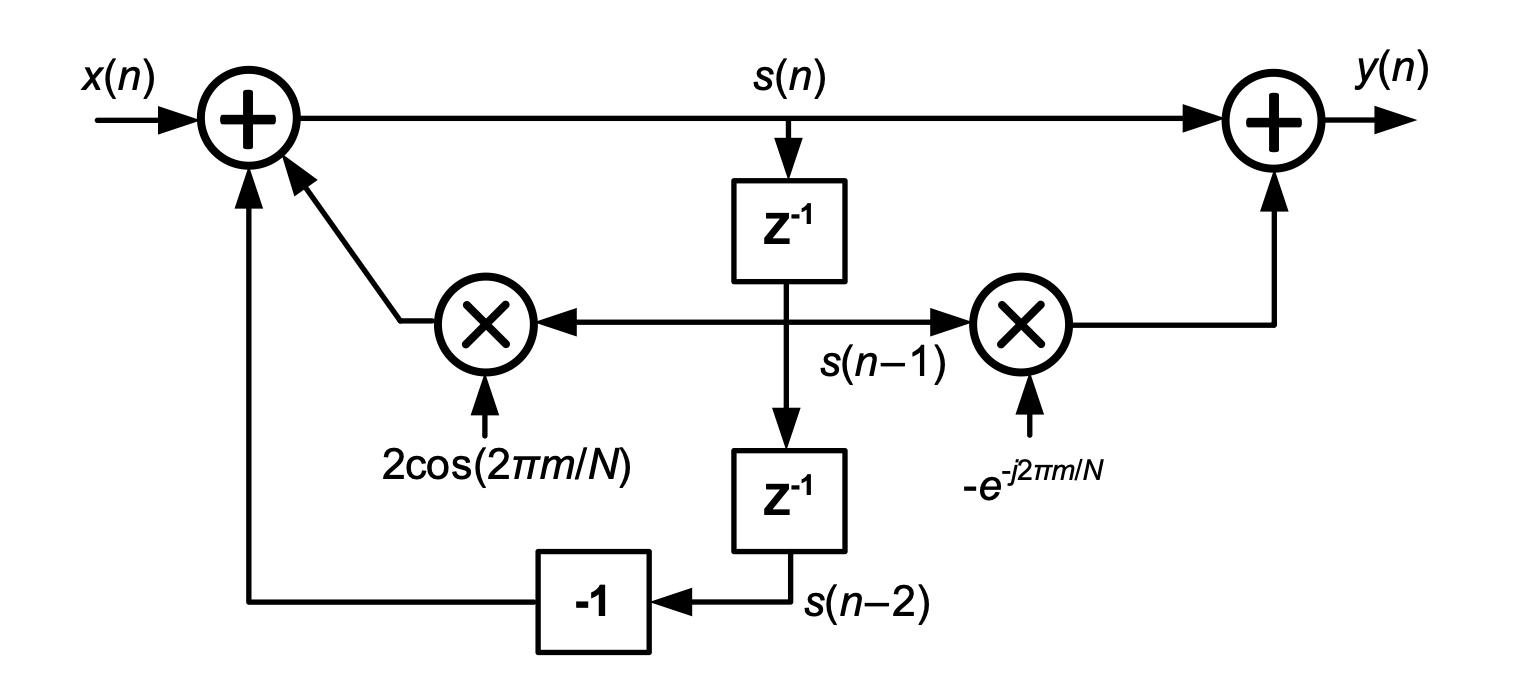
\includegraphics[width = 12cm]{img/gf_overview.png}
    \caption{IIR filter structure of the Goertzel algorithm. \cite{9464344}}
    \label{fig:gf_overview}
\end{figure}